\section{DATASET}
\subsection{Data exploration}
Il dataset fornito presenta $858$ record, ognuno associato ad un totale di $36$ valori, etichetta inclusa. Un elenco degli attributi presenti nel dataset è riportata in Tabella \ref{tab:attributes}, dove viene altresì riportato il DataType associato ad ognuno di essi. I dati provengono da uno screening effettuato su una popolazione di donne in un ospedale di Caracas, Venezuela \todo{cita sito}, delle quali sono stati raccolti e riportati una serie di dati personali, medici e strumentali. In particolare, nel dataset è possibile individuare un gruppo di attributi relativi all'attività sessuale delle donne, al numero di partner ed al tipo di contraccettivo utilizzato (ormonale vs intrauterino - IUD -). Viene poi riportata una lunga lista di malattie sessualmente trasmissibili (STDs), il numero totale di patologie sessuali contratte e l'intervallo di tempo trascorso dalla prima e dall'ultima diagnosi di queste malattie. Sono infine presenti informazioni circa precedenti diagnosi di cancro o Papilloma Virus (DX) e i risultati di alcuni esami strumentali eseguiti sulle pazienti. L'attributo etichetta, ovvero quello su cui il modello di predizione proposto si è concertato, è l'esito della Biopsia, un esame eseguito su una porzione del tessuto sospetto in di accertare la presenza o meno di cellule tumorali attive. 
\begin{table}
	\centering
	\caption{Tabella riportante gli attributi presenti nel dataset ed il relativo tipo.
	\todo[inline]{Credo che, per come è stato fatto il corso, sia più corretto mettere nominale, ordinale, intervallo, ratio al posto del "tipo programmativo". DP}}
	\label{tab:attributes}
	\begin{tabular}{|c|c|}
		\toprule 
		Attributo & DataType \\ 
		\midrule 
		Age & Int \\ 
		Number of sexual partners & Int \\ 
		First sexual intercourse & Int \\ 
		Num of pregnancies & Int \\  
		Smokes & Bool \\  
		Smokes (years) & Double \\ 
		Smokes (packs/year) & Double \\ 
		Hormonal Contraceptives & Bool \\ 
		Hormonal Contraceptives (years) & Double \\ 
		IUD & Bool \\ 
		IUD (years) & Double \\ 
		STDs & Bool \\ 
		STDs (number) & Int \\ 
		STDs:condylomatosis & Bool \\ 
		STDs:cervical condylomatosis & Bool \\ 
		STDs:vaginal condylomatosis & Bool \\ 
		STDs:vulvo-perineal condylomatosis & Bool \\ 
		STDs:syphilis & Bool \\ 
		STDs:pelvic inflammatory disease & Bool \\ 
		STDs:genital herpes & Bool \\ 
		STDs:molluscum contagiosum & Bool \\ 
		STDs:AIDS & Bool \\ 
		STDs:HIV & Bool \\ 
		STDs:Hepatitis B & Bool \\ 
		STDs:HPV & Bool \\ 
		STDs: Number of diagnosis & Int \\  
		STDs: Time since first diagnosis & Double \\ 
		STDs: Time since last diagnosis & Double \\ 
		Dx:Cancer & Bool \\ 
		Dx:CIN & Bool \\ 
		Dx:HPV & Bool \\ 
		Dx & Bool \\ 
		Hinselmann & Bool \\ 
		Schiller & Bool \\  
		Citology & Bool \\ 
		Biopsy & Bool \\ 
		\bottomrule 
	\end{tabular} 
\end{table}

L'analisi del dataset ha quindi analizzato la natura del problema di classificazione da affrontare. Lo studio della distribuzione delle etichette ha riportato un forte sbilanciamento delle classi, come rappresentato in Figura \ref{fig:biopsydistribution}, con solo $55$ record ($6,4\%$ del totale) appartenenti alla classe positiva.
\begin{figure}
	\centering
	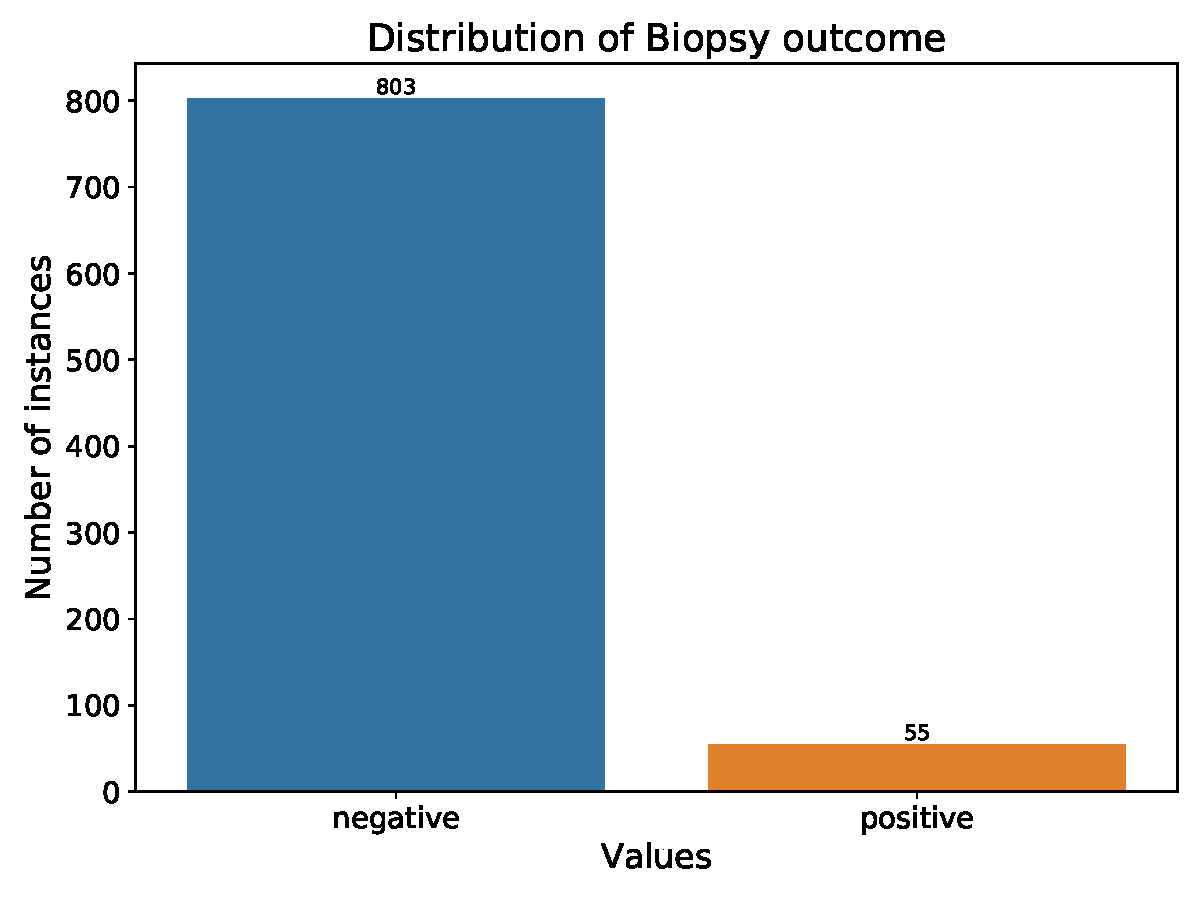
\includegraphics[width=0.8\linewidth]{images/biopsy_distribution}
	\caption{Distribuzione delle etichette all'interno del dataset. Il problema risulta fortemente sbilanciato verso la classe negativa.}
	\label{fig:biopsydistribution}
\end{figure}
A seguito della fase di \textit{Data cleaning}, presentata nella sottosezione successiva, è stato eseguito uno studio della correlazione tra i vari attributi del dataset (inclusa l'etichetta). La Figura \ref{fig:corrmatrix} riporta la \textit{heatmap} associata ai valori di correlazione; da essa si evince la presenza di una forte correlazione interna tra gli attributi relativi alle malattie sessualmente trasmissibili e tra gli esami di laboratorio e l'etichetta. Più in generale, è presente una correlazione elevata tra quelle coppie di attributi che rappresentano il medesimo dato, in un caso tramite valore booleano, nell'altro mediate dato numerico. Questa costatazione risulta in linea con le aspettative e suggerisce una presenza di ridondanza dell'informazione, risolvibile mediante l'utilizzo di tecniche di riduzione della dimensionalità.
\begin{figure}
	\centering
	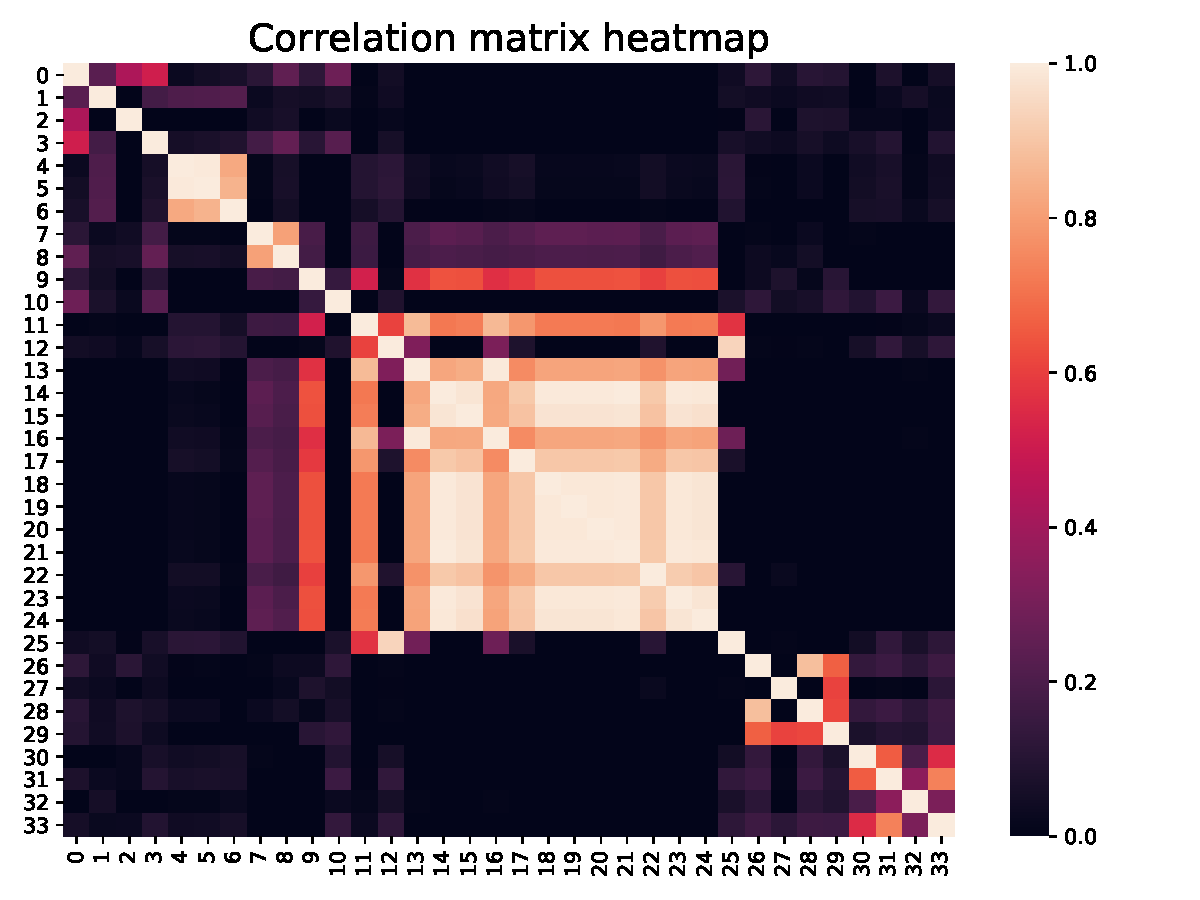
\includegraphics[width=0.8\linewidth]{images/corr_matrix}
	\caption{Matrice di correlazione degli attributi del dataset. Legenda:
		0) Age,
		1) Number of sexual partners,
		2) First sexual intercourse,
		3) Num of pregnancies,
		4) Smokes,
		5) Smokes (years),
		6) Smokes (packs/year),
		7) Hormonal Contraceptives,
		8) Hormonal Contraceptives (years),
		9) IUD,
		10) IUD (years),
		11) STDs,
		12) STDs (number),
		13) STDs:condylomatosis,
		14) STDs:cervical condylomatosis,
		15) STDs:vaginal condylomatosis,
		16) STDs:vulvo-perineal condylomatosis,
		17) STDs:syphilis,
		18) STDs:pelvic inflammatory disease,
		19) STDs:genital herpes,
		20) STDs:molluscum contagiosum,
		21) STDs:AIDS,
		22) STDs:HIV,
		23) STDs:Hepatitis B,
		24) STDs:HPV,
		25) STDs: Number of diagnosis,
		26) Dx:Cancer,
		27) Dx:CIN,
		28) Dx:HPV,
		29) Dx,
		30) Hinselmann,
		31) Schiller,
		32) Citology,
		33) Biopsy.}
	\label{fig:corrmatrix}
\end{figure}


\subsection{Data cleaning and preprocessing}
È stata dapprima indagata la presenza di valori mancanti nel dataset, rilevando come i due attributi relativi alla data della prima e ultima diagnosi di malattie sessualmente trasmissibili presentassero un numero elevatissimo di valori nulli; per questo motivo è stato deciso di rimuovere dal dataset questi dati, in quanto un tentativo di imputazione di questi valori si sarebbe dovuto basare su un numero di sample davvero esiguo. Non è invece stata rilevata la presenza di record con un elevato numero di attributi mancanti.
Il dataset è stato quindi diviso secondo l'etichetta ed è stata applicata una tecnica di imputazione per i \textit{missing value} dei due sottogruppi così generati: gli attributi interi sono stati sostituiti con la mediana dei valori, quelli booleani con il valore più frequente mentre per i valori continui è stata utilizzato il valore medio arrotondato a intero. Quest'ultima scelta è stata presa a seguito dell'analisi qualitativa dei dati, che ha mostrato come la stragrande maggioranza dei valori contenuti negli attributi Double risultasse essere pari a 0 o ad un valore intero. Per questo motivo, al fine di non introdurre un'alterazione nel tipo dei dati presenti, è stata preferita una media arrotondata ad una più classica media semplice.
Dopo aver riunito il dataset, è stata effettuata una ricerca di outlier statistici; per fare ciò sono stati considerati unicamente gli attributi relativi all'età delle pazienti e ai dati sull'attività sessuale. Non sono stati inclusi attributi circa le abitudini di consumo di sigarette o i dati relativi agli anticoncezionali in quanto l'elevato numero di record con valori associati a questi attributi pari a $0$ avrebbe portato a considerare la maggioranza delle istanze con valori non nulli in questi campi degli outlier. A seguito della rimozione dei valori che superavano in uno degli attributo considerati tre volte il range interquantile, il dataset presenta un totale di 776 esempi per la classe negativa e 54 esempi per la classe positiva, evidenziando come la maggioranza degli outlier sia stata individuata nella classe negativa.